\documentclass[../dissertation.tex]{subfiles}
\begin{document}
Now that gradient flow equation and tangent-point energy are introduced,
one can formalise the process of untangling a tangled curve:

\begin{definition}[Curve Untangling Process]
    Given a parameterised curve $\gammabf:M \times T \rightarrow \mathbb{R}^3$ over an interval $M$ and time domain $T$,
    denote the following initial value problem as \textbf{curve untangling process}:
    \begin{align}
        \frac{\partial \gammabf}{\partial t} &= - \grad_{\mathcal{X}} \mathcal{E}_{\beta}^{\alpha} (\gammabf) - \grad_{\mathcal{X}} \mathcal{C} (\gammabf) 
        \label{equ: Curve Untangling Process}
        \\
        \gammabf(s;0) &= \gammabf_0 (s)
        \label{equ: Initial Curve}
    \end{align}
    where 
    \begin{itemize}
        \item $\gammabf_0 (s)$ is the parameterisation of the initial (tangled) curve (prescribed at $t=0$)
        \item $\mathcal{E}_{\beta}^{\alpha}$ is the tangent-point energy (See (\ref{equ: Tangent-Point Energy}))
        \item $\mathcal{C}$ is additional constraint energy to control behaviour of curve untangling process.
    \end{itemize}
\end{definition}

\subsection{Discretisation for Numerical Computation}
Solving (\ref{equ: Curve Untangling Process}), (\ref{equ: Initial Curve}) analytically is challenging.
Rather, we aim to acquire a numerical solution.
Assume for simplicity that the curve of interest is closed.\footnote{
    We may assume that the function definition of $\gammabf:M \rightarrow \mathbb{R}^3$ extends to $\gammabf: \mathbb{R} \rightarrow \mathbb{R}^3$ by periodicity.
}

\subsubsection{Discretisation of Curve}
We start by discretising the initial curve $\gammabf_0$ by taking $N$ points on a curve as shown in Figure \ref{fig: Discretization of Curve}.
Represent the initially discretised curve as $\Gammabf^0 = \left( \xbf_0^0, \xbf_1^0, \cdots, \xbf_{N-1}^0 \right)$,
and the discretised curve at time step $k \in \mathbb{N} \cup \left\{ 0 \right\}$ as $\Gammabf^k = \left( \xbf_0^k, \xbf_1^k, \cdots, \xbf_{N-1}^k \right)$.
Since we restrict our attention to a closed curve, it is convenient to extend the indexing rule by:
\begin{equation}
    \xbf_{i}^k = \xbf_{r\left( i,N \right)}^k \hspace{1cm} \text{where } r\left( i,N \right) = \text{(remainder of } i \div N \text{)}
\end{equation}
so that $\xbf_N^k = \xbf_{0}^k$, $\xbf_{N+1}^k = \xbf_{1}^k$, etc.

Assign a function definition $\Gammabf^k: \mathbb{Z} \rightarrow \left\{ \xbf_0^k, \xbf_1^k, \cdots, \xbf_{N-1}^k \right\}$ as:
\begin{equation}
    \Gammabf^k (i) = \xbf_{r\left( i, N \right)}^k 
\end{equation}
anaogous to $\gammabf = \gammabf(s)$ being a parameterised curve, which is a vector-valued function.

Finally, denote by $e_{i}^k$ for the (undirected) edge with vertex pair $\left( \xbf_i^k, \xbf_{i+1}^k \right)$.

\subsubsection{Discretisation of Tangent-Point Energy}
Note that $\Gammabf^k$ is a polygonal curve, for which tangent-point energy (\ref{equ: Tangent-Point Energy}) is not well-defined due to locally non-integrable contributions from vertices:

\begin{figure}[tbp]
    \centering
    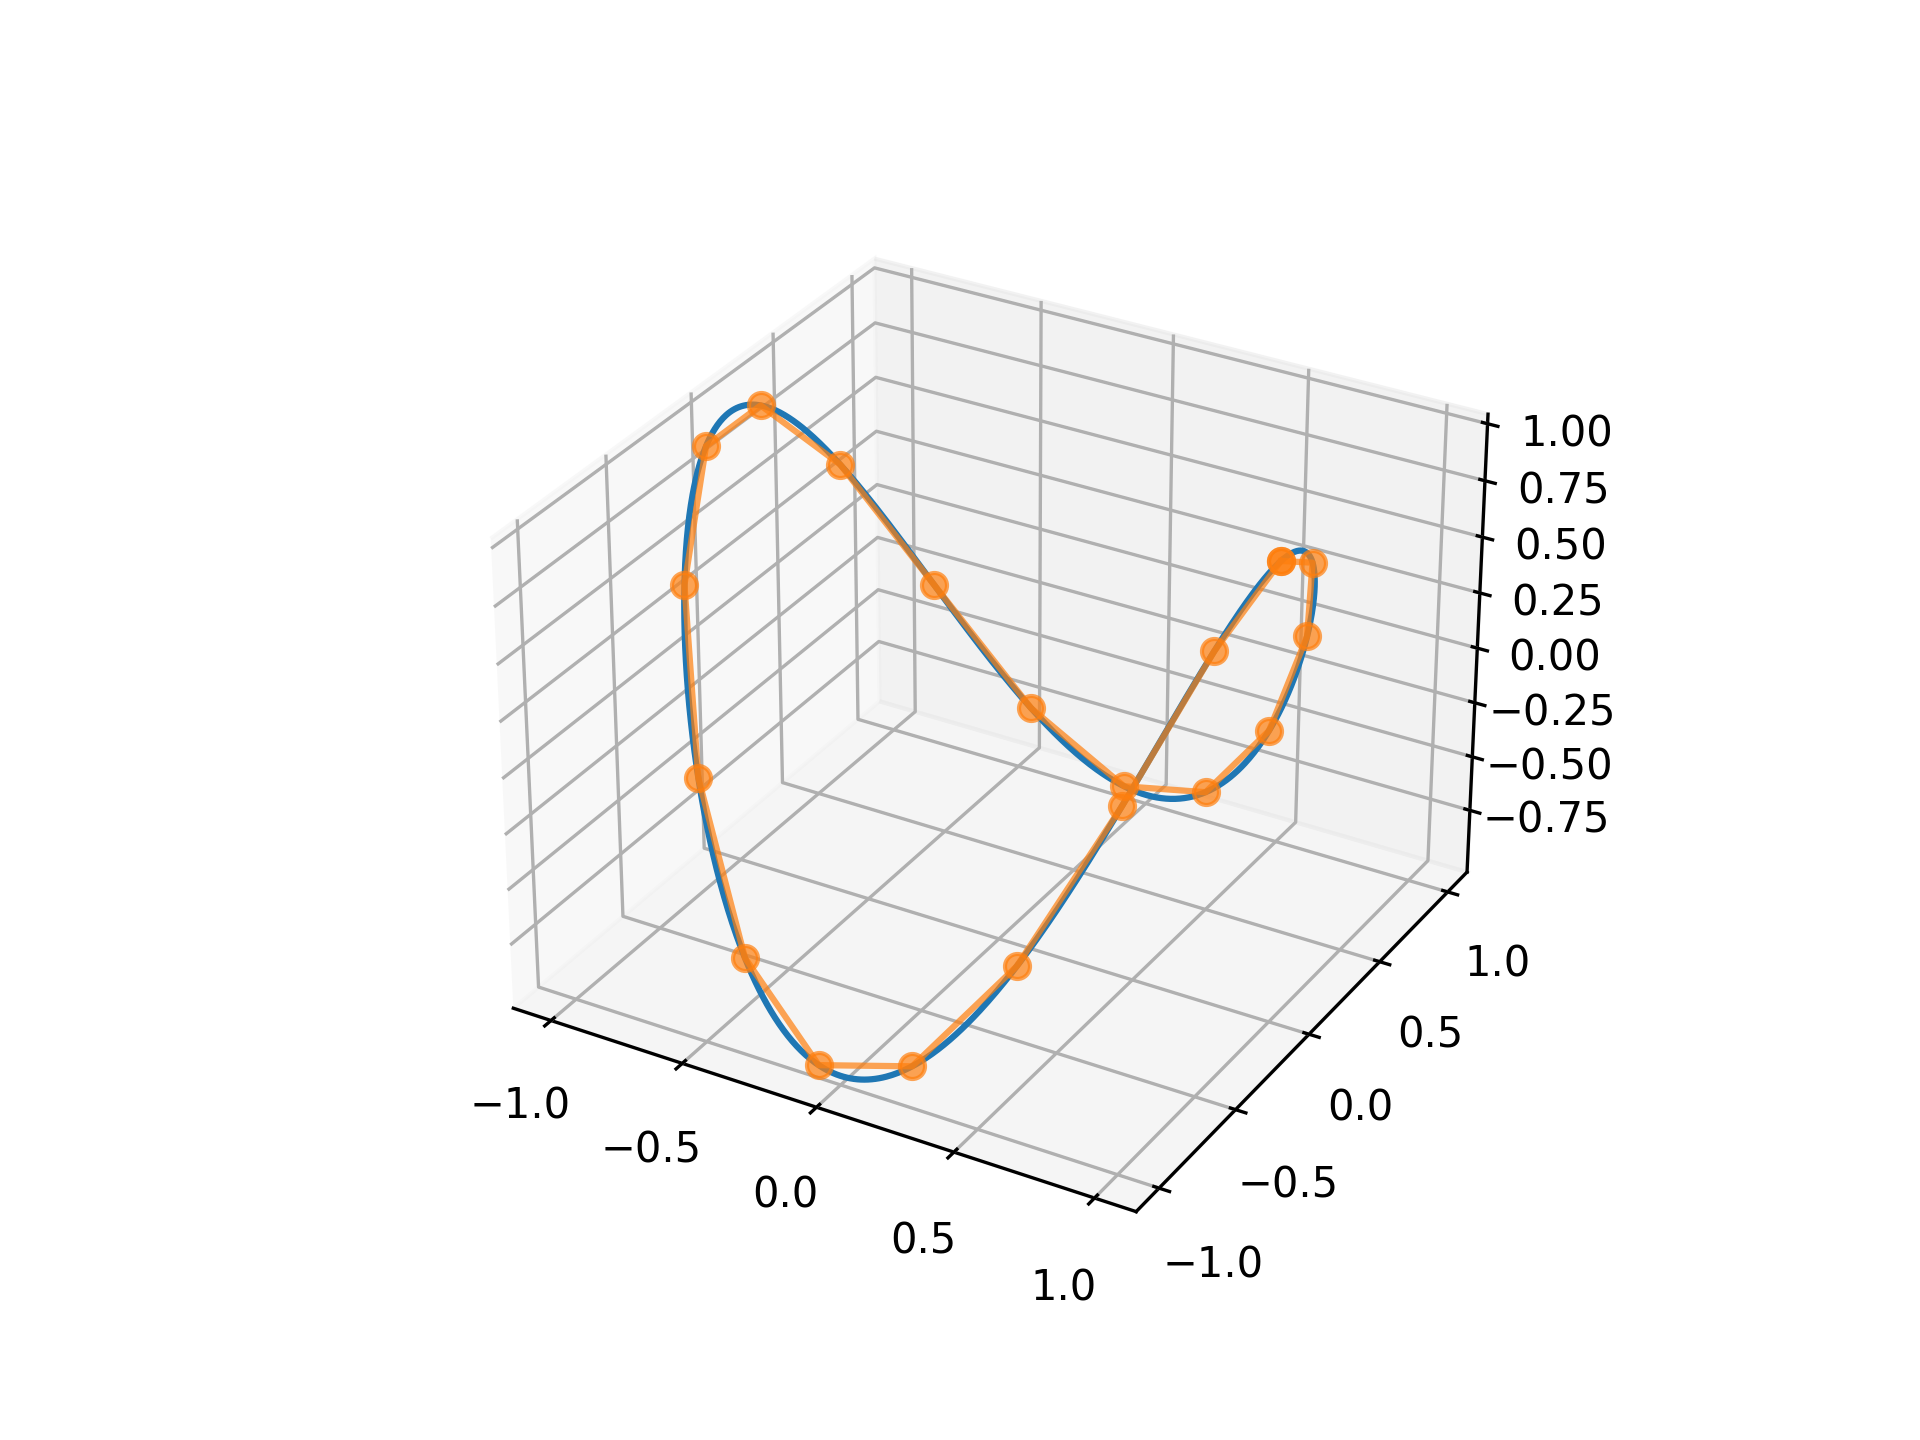
\includegraphics[width=0.8\textwidth]{sections/discretizationImgs/discretization}
    \caption{Discretisation of a closed curve by sampling the points along the curve.}
    \label{fig: Discretization of Curve}
\end{figure}

One way to resolve the issue is to ``ignore'' the adjacent edge contribution in the energy quadrature $E_{\beta}^{\alpha}$ as shown in Figure \ref{fig: Energy discretization by ignoring adjacent edges}.
\begin{figure}[tbp]
    \centering
    \begin{subfigure}[b]{0.8\textwidth}
        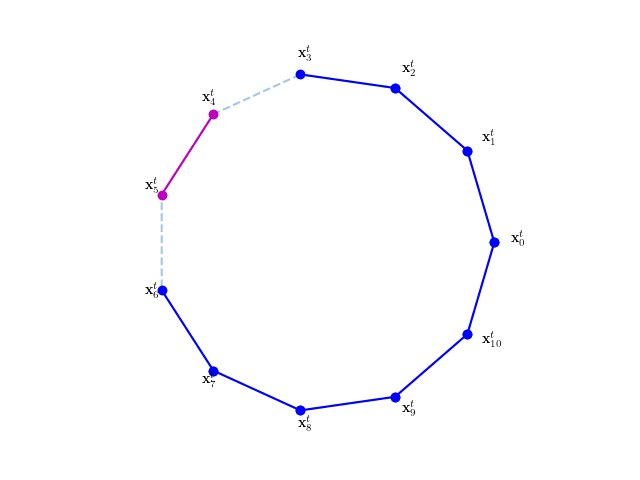
\includegraphics[width=\textwidth]{sections/unknottingCurveImgs/energyDiscretization1}
        \caption{For a chosen edge $e_i^k$, ignore the two adjacent edges $e_{i-1}^k$, $e_{i+1}^k$.
            In the limit as $N \rightarrow 0$, because the edge lengths tend to zero,
            the discrepancy between the quadrature and the analytical value of the energy is expected to tend to zero.
                }
        \label{fig: Energy discretization by ignoring adjacent edges}
    \end{subfigure}
    \par\bigskip
    \begin{subfigure}[b]{0.8\textwidth}
        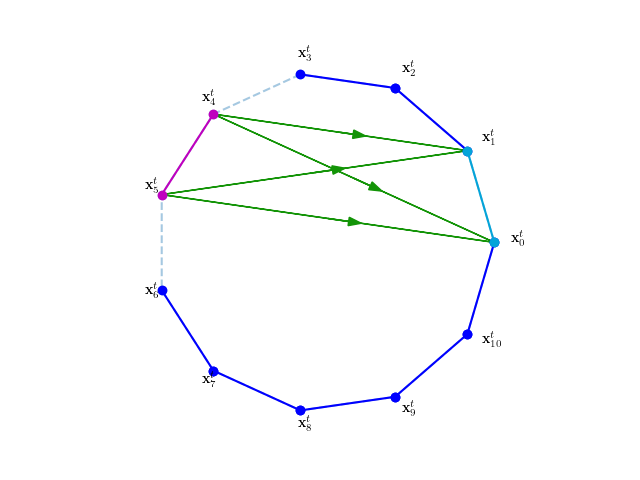
\includegraphics[width=\textwidth]{sections/unknottingCurveImgs/energyDiscretization2}
        \caption{Tangent-point kernel is approximated by 4-point quadrature.}
        \label{fig: Tangent-point kernel approximation}
    \end{subfigure}
    \caption{Quadrature for approximation of tangent-point energy.}
\end{figure}

\subsubsection{Finite Difference Scheme of Curve Untangling Process}
Based on (\ref{equ: Curve Untangling Process}), one writes the following finite difference scheme:
\begin{equation}
    \mathcal{D}_{t} \Gammabf^{k} = -\grad_{\mathcal{X}} E_{\beta}^{\alpha} (\Gammabf^k) - \grad_{\mathcal{X}} C \left( \Gammabf^k \right) \hspace{1cm} \text{for } k=0,1,\cdots
\end{equation}
where $\mathcal{D}_t$ is the finite difference operator over time step.
For the simplest scheme, one could take the forward difference operator as $\mathcal{D}_t \Gammabf^k(i) \coloneqq \frac{\Gammabf^{k+1}(i) - \Gammabf^{k}(i)}{\Delta T}$.

\subsection{$L^2$ Explicit Euler Scheme}

\end{document}
